\chapter{Work Experience} % Main chapter title

\label{Chapter2} % Change X to a consecutive number; for referencing this chapter elsewhere, use \ref{ChapterX}

\lhead{Chapter 2. \emph{Work Experience}} % Change X to a consecutive number; this is for the header on each page - perhaps a shortened title

I have had a total of six work placements since the start of my gap year.
Figure \ref{timeline} provides a timeline of the companies I have worked at.
The focus of this chapter will be on my placement at Sunamp, which was specifically done as part of D11PJ \textit{Industrial Project}.
After describing my experience at Sunamp, I will briefly describe my other work experiences.

\begin{figure}[htbp]
	\centering
	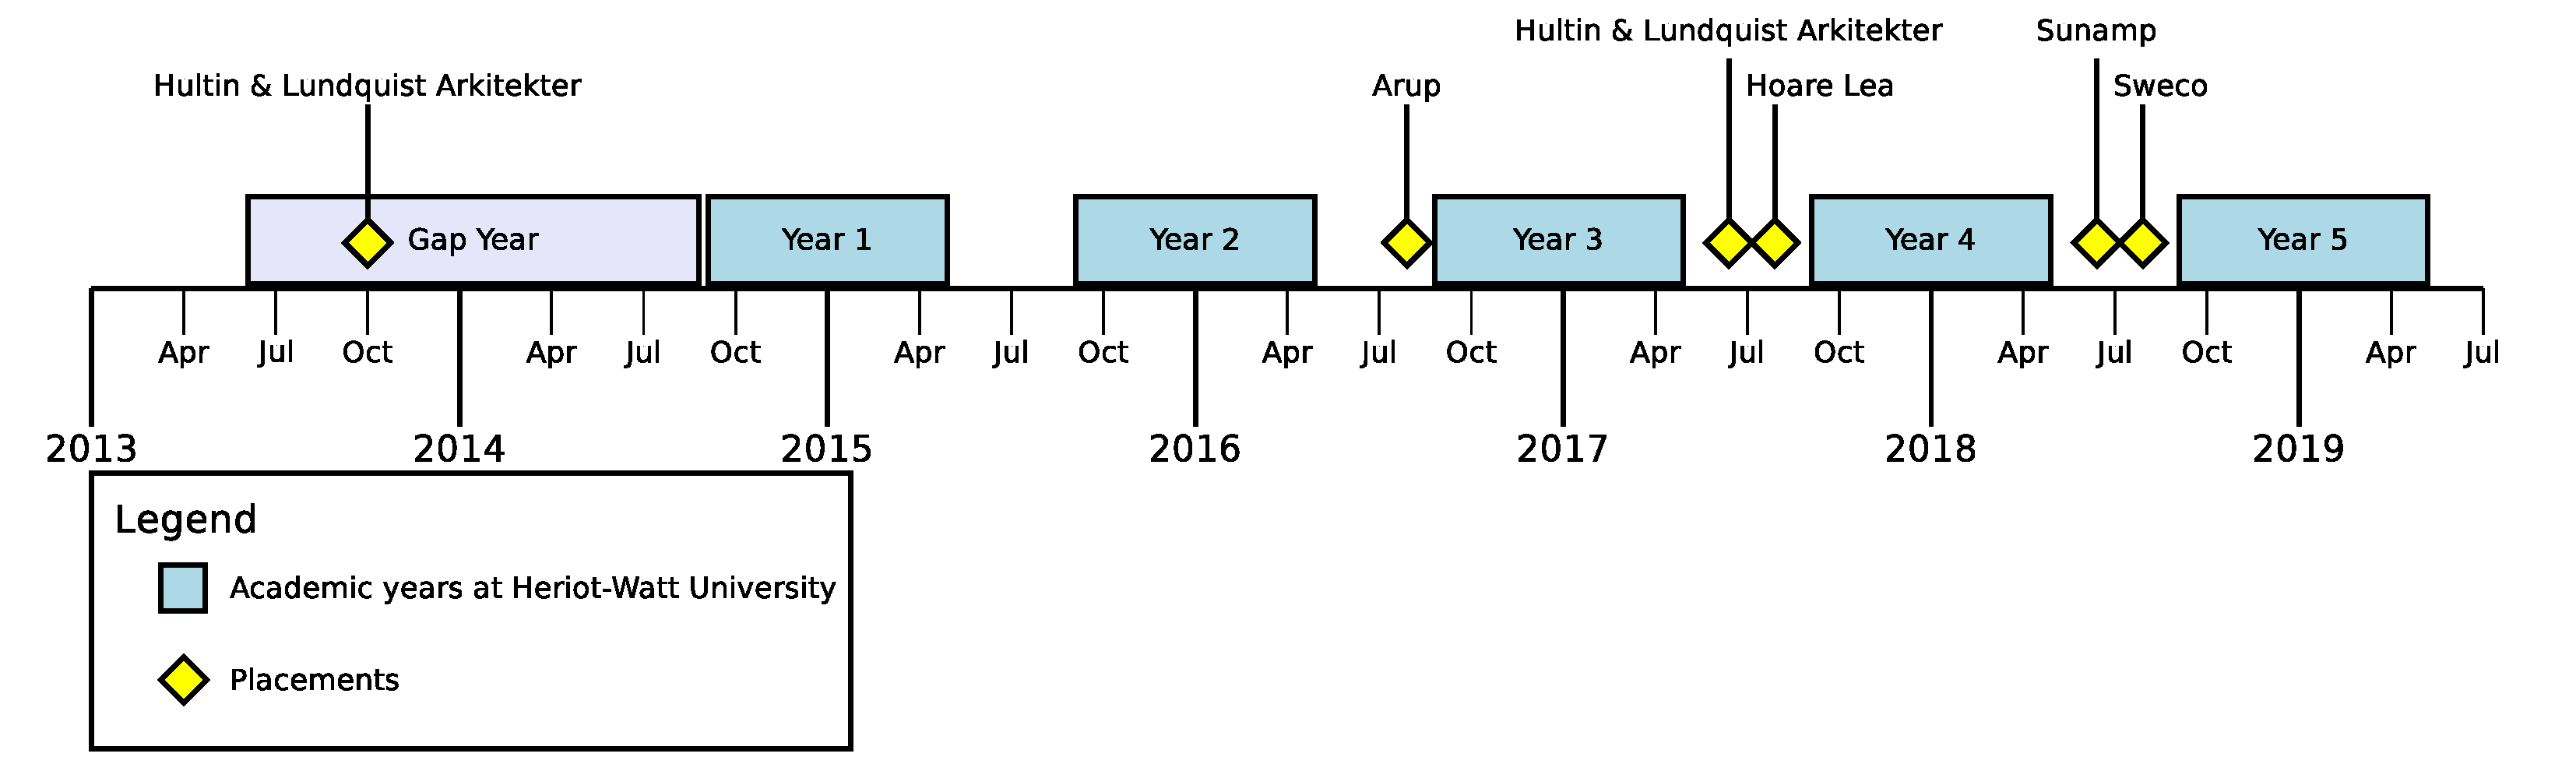
\includegraphics[width=\textwidth]{figures/IP-Timeline.eps}
	\rule{\textwidth}{0.5pt} % use line???
	\caption{Timeline of my work placements since my pre-university gap year.}
	\label{timeline}
\end{figure}


%----------------------------------------------------------------------------------------
%	SECTION 1
%----------------------------------------------------------------------------------------

\section{Sunamp, July - August 2018}

My placement at Sunamp started on 3\textsuperscript{rd} July 2018 and ended on 10\textsuperscript{th} August 2018.
I worked a total of 198 hours there (\hl{see time/ work log in Appendix ...}).


\subsection{Application Process}

I learned about the opportunity of two paid placements with immediate start at Sunamp through David Campbell, the D11PJ course leader.
He had asked applicants for this placement to send him 100 words broadly describing their strengths and preferences, which he would then forward to Sunamp.
A coursemate named Hamish and I were both interested in this opportunity.
\hl{My hundred-word application went as follows:}

Strengths:
\begin{itemize}
	\item I am very familiar with the BIM process, having written a dissertation on collaboration with regards to BIM.
	\item I have work experience in mechanical and electrical consulting engineering.
	\item Organised, flexible, independent and cooperative.
\end{itemize}
Skills:
\begin{itemize}
	\item Advanced skills in Microsoft Office packages and Bluebeam Revu.
	\item Intermediate skills in LaTeX.
	\item Basic modelling skills in Revit, AutoCAD and IES-VE.
	\item Fluent in three languages (English, Swedish and French) with basic knowledge of Spanish.
\end{itemize}
Preferences/ interests:
\begin{itemize}
	\item Highly interested in learning about your application of Phase Change Materials in thermal storage batteries.
	\item Also interested in working with BIM and learning Bentley’s Hevacomp software packages.
\end{itemize}

After the applications, David introduced us applicants to Susan Lang-Bissell, the Managing Director (MD) of Sunamp, via email.
David had asked us to liaise with Susan to arrange a meeting.
To do this, Hamish and I first established our availabilities in the upcoming days.
I then volunteered to liaise with Susan via email on our behalf to find a suitable date and time.

\hl{Try to be more reflective, and less descriptive.
Maybe record (vocally) the story, and then reflect on it out loud. THEN write about it.}